% Generated by jats2tex@0.11.1.0
\documentclass{article}
\usepackage[T1]{fontenc}
\usepackage[utf8]{inputenc} %% *
\usepackage[portuges,spanish,english,german,italian,russian]{babel} %% *
\usepackage{amstext}
\usepackage{authblk}
\usepackage{unicode-math}
\usepackage{multirow}
\usepackage{graphicx}
\usepackage{etoolbox}
\usepackage{xtab}
\usepackage{enumerate}
\usepackage{hyperref}
\usepackage{penalidades}
\usepackage[footnotesize,bf,hang]{caption}
\usepackage[nodayofweek,level]{datetime}
\usepackage[top=0.85in,left=2.75in,footskip=0.75in]{geometry}
\newlength\savedwidth
\newcommand\thickcline[1]{\noalign{\global
\savedwidth
\arrayrulewidth
\global\arrayrulewidth 2pt}
\cline{#1}
\noalign{\vskip\arrayrulewidth}
\noalign{\global\arrayrulewidth\savedwidth}}
\newcommand\thickhline{\noalign{\global
\savedwidth\arrayrulewidth
\global\arrayrulewidth 2pt}
\hline
\noalign{\global\arrayrulewidth\savedwidth}}
\usepackage{lastpage,fancyhdr}
\usepackage{epstopdf}
\pagestyle{myheadings}
\pagestyle{fancy}
\fancyhf{}
\setlength{\headheight}{27.023pt}
\lhead{
\includegraphics[width=10mm]{logo.png}}
\rhead{\ifdef{\journaltitle}{\journaltitle}{}
\ifdef{\volume}{vol.\,\volume}{}
\ifdef{\issue}{(\issue)}{}
\ifdef{\fpage}{\fpage--\lpage\,pp.}}
\rfoot{\thepage/\pageref{LastPage}}
\renewcommand{\footrule}{\hrule height 2pt \vspace{2mm}}
\fancyheadoffset[L]{2.25in}
\fancyfootoffset[L]{2.25in}
\lfoot{\sf \ifdef{\articledoi}{\articledoi}{}}
\setmainfont{Linux Libertine O}
\renewcommand*{\thefootnote}{\alph{footnote}}
\makeatletter
\newcommand{\fn}{\afterassignment\fn@aux\count0=}
\newcommand{\fn@aux}{\csname fn\the\count0\endcsname}
\makeatother

\newcommand{\journalid}{Bull World Health Organ}
\newcommand{\journaltitle}{Bulletin of the World Health Organization}
\newcommand{\abbrevjournaltitle}{Bull. World Health Organ.}
\newcommand{\issnppub}{0042-9686}
\newcommand{\publishername}{World Health Organization}
\newcommand\articleid{\textsc{blt}.13.021113}
\newcommand\articledoi{\textsc{doi} 10.2471/\textsc{blt}.13.021113}
\def\subject{News}\newcommand{\subtitlestyle}[1]{-- \emph{#1}\medskip}
\newcommand{\transtitlestyle}[1]{\par\medskip\Large #1}
\newcommand{\transsubtitlestyle}[1]{-- \Large\emph{ #1}}

\newcommand{\titlegroup}{
\ifdef{\subtitle}{\subtitlestyle{\subtitle}}{}
\ifdef{\transtitle}{\transtitlestyle{\transtitle}}{}
\ifdef{\transsubtitle}{\transsubtitlestyle{\transsubtitle}}{}}

\title{More midwives needed to improve maternal and newborn
survival\titlegroup{}}
\date{ 11 2013}
\def\volume{91}
\def\issue{11}
\def\fpage{804}
\def\lpage{805}
\def\permissions{(c) World Health Organization (\textsc{who}) 2013. All rights
reserved.2013}

\begin{document}
\selectlanguage{english}
\section*{Metadados não aplicados}
\begin{itemize}
\item[\textbf{língua do artigo}]{Inglês}
\ifdef{\journalid}{\item[\textbf{journalid}] \journalid}{}
\ifdef{\journaltitle}{\item[\textbf{journaltitle}] \journaltitle}{}
\ifdef{\abbrevjournaltitle}{\item[\textbf{abbrevjournaltitle}]
\abbrevjournaltitle}{}
\ifdef{\issnppub}{\item[\textbf{issnppub}] \issnppub}{}
\ifdef{\issnepub}{\item[\textbf{issnepub}] \issnepub}{}
\ifdef{\publishername}{\item[\textbf{publishername}] \publishername}{}
\ifdef{\publisherid}{\item[\textbf{publisherid}] \publisherid}{}
\ifdef{\subject}{\item[\textbf{subject}] \subject}{}
\ifdef{\transtitle}{\item[\textbf{transtitle}] \transtitle}{}
\ifdef{\authornotes}{\item[\textbf{authornotes}] \authornotes}{}
\ifdef{\articleid}{\item[\textbf{articleid}] \articleid}{}
\ifdef{\articledoi}{\item[\textbf{articledoi}] \articledoi}{}
\ifdef{\volume}{\item[\textbf{volume}] \volume}{}
\ifdef{\issue}{\item[\textbf{issue}] \issue}{}
\ifdef{\fpage}{\item[\textbf{fpage}] \fpage}{}
\ifdef{\lpage}{\item[\textbf{lpage}] \lpage}{}
\ifdef{\permissions}{\item[\textbf{permissions}] \permissions}{}
\end{itemize}
\maketitle

\begingroup

\begin{abstract}

Retention of midwives, especially in rural areas, is a major challenge for many
countries, one
that threatens to negate all the hard work and resources invested in their
training. Priya Shetty
reports.

\iflanguage{portuges}{\medskip\noindent\textbf{Palavras-chave:} \kwdgroup}{}
\iflanguage{english}{\medskip\noindent\textbf{Keywords:} \kwdgroupen}{}
\iflanguage{spanish}{\medskip\noindent\textbf{Palavras claves:} \kwdgroupes}{}
\iflanguage{french}{\medskip\noindent\textbf{Mots clés:} \kwdgroupfr}{}
\end{abstract}
\endgroup

“They are often accommodated in the most awful insanitary conditions, with no
running
water and these conditions are not limited to isolated rural areas. What's
worse, it may be
unsafe, especially for those doing 24-hour shifts.” Frances McConville,
midwifery expert at
the World Health Organization (\textsc{who}) in Geneva, is not describing soldiers, but
midwives in some of
the world's poorest and most unstable regions.

In a way, these health workers are the warriors on the front-line of health
care, battling to
ensure that women survive childbirth and that babies are born safely even in the
most marginalized
areas.

Midwifery, a practice so ancient that it features in early Egyptian and Roman
scrolls, is seeing
a long awaited increase in global attention. Decades of neglect of the role of
midwives, either
because of the over-medicalization of pregnancy care or a lack of resources, has
left a legacy of
high rates of maternal and newborn mortality in developing countries. While
these rates have fallen
in recent years, more progress must be made in Asia and sub-Saharan Africa,
where fewer than 50\% of
all births are assisted by a skilled birth attendant.

Now, grassroots, government and international initiatives are coming together to
put midwives at
centre stage in reproductive health programmes in countries like Ethiopia and
Somalia. But for these
efforts to succeed, investment in midwifery must be sustainable, covering more
than just the initial
training.
\begin{figure}
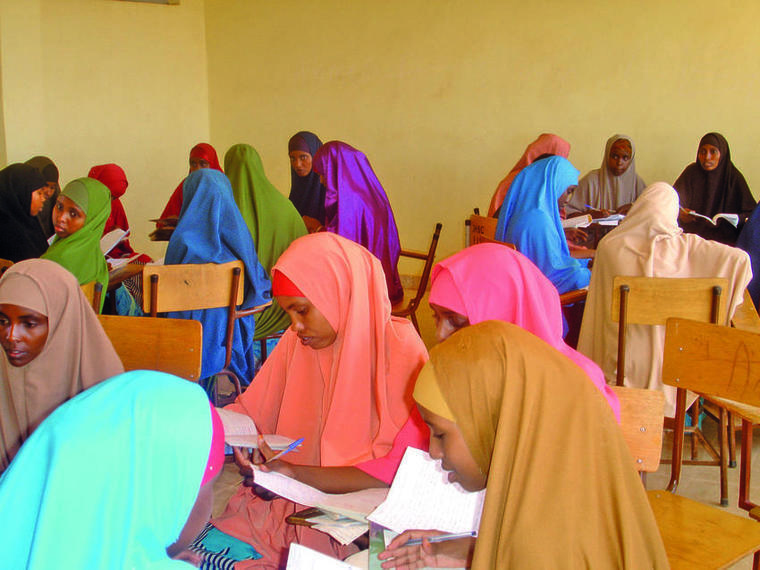
\includegraphics[width=\textwidth]{0042-9686-bwho-91-11-804-Fa}
\caption{}\label{fig:Fa}
\end{figure}

In 2011, the United Nations Population Fund (\textsc{unfpa}) published a report –
\textit{The state
of the world's midwifery 2011: delivering health, saving lives}
– that offered a
comprehensive look at midwifery around the globe. The report was “incredibly
revealing” says McConville. Its analysis of 58 countries showed that there was a
global
shortage of an estimated 350 000 midwives, at least a third of whom were needed
in the
world's poorest countries.

Regional efforts to improve midwifery have increased with the launch this year
of the
Confederation of African Midwives Associations to advocate for better education
and regulation of
midwives.

Midwifery has come to the fore since maternal and newborn health were made the
focus of two of
the Millennium Development Goals (\textsc{mdg}s). And there is another reason for renewed
attention: the
world is facing an acute shortage of health-care workers. Overall, \textsc{who} estimated
in 2006 that the
world needs 4.2 million more health workers, with 1.5 million of those needed in
African countries
alone.

Increasing the number of skilled health workers is even more important now that
countries are
striving towards universal health coverage. The growing support for task
shifting, in which duties
are redistributed so that doctors and nurses are not overburdened, has also
created a greater demand
for workers with midwifery skills, says McConville.

However, midwifery experts say that for a profession that is so old, it is
remarkably poorly
understood. “Midwives do far more than just catch babies,” says Petra ten
Hoope-Bender, a director for reproductive, maternal, newborn and child health at
the
\textit{Instituto de Cooperación Social Integrare}, a research institute in Spain.
The impact midwives have is not just on pregnancy outcomes, as is often assumed,
she says, but
extends to newborn care, breastfeeding, family planning, and sometimes also
cervical and breast
cancer screening.

Nevertheless, “in developing countries especially, midwives are often at the
bottom of the
ladder of the health system,” says ten Hoope-Bender. She argues that midwives
should be at
the heart of the continuum of care, whether in terms of screening women for \textsc{hiv}
infection,
tuberculosis and malaria or of detecting early signs of noncommunicable diseases
through routine
antenatal checks, such as measuring blood pressure and testing for diabetes.
\begin{figure}
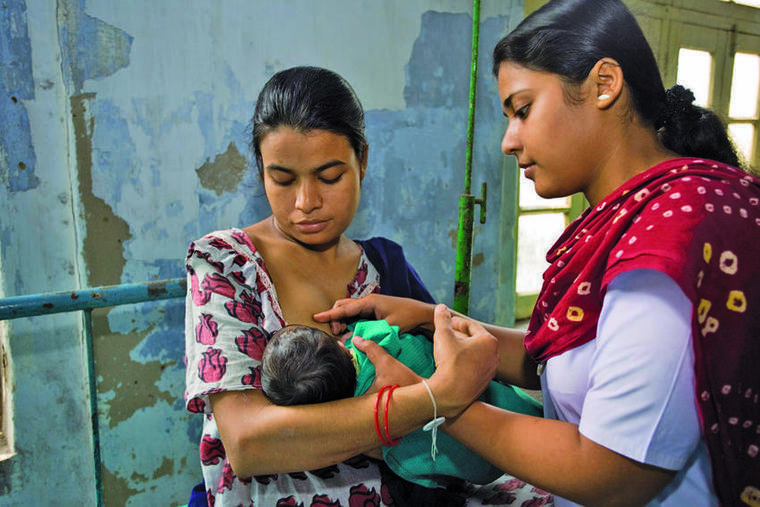
\includegraphics[width=\textwidth]{0042-9686-bwho-91-11-804-Fb}
\caption{}\label{fig:Fb}
\end{figure}

The linkages with infectious and chronic diseases could allow midwifery
programmes to seek
funding from \textsc{hiv} infection or tuberculosis programmes, for instance, says Dr Luc
de Bernis, senior
maternal health adviser at \textsc{unfpa}, who is coordinating the development of the
\textit{State of the
world's midwifery 2014}
report.

Another reason why midwifery has been sidelined, says ten Hoope-Bender, is the
focus on emergency
obstetric care and facility-based childbirth, which have been at the heart of
efforts to achieve the
\textsc{mdg}s. But “when midwifery is in place, there is much less need for emergency
interventions
because problems requiring prompt attention are managed or referred before they
become a
life-threatening complication,” she says.

“When midwifery is in place, there is much less need for emergency
interventions.”
Petra ten Hoope-Bender
Training is now a major focus in midwifery, and – for women in poor countries –
the
new generation of midwives can't come soon enough. This is essential in Somalia,
where a
woman has a 1 in 16 chance of survival beyond her reproductive years. According
to Achu Lordfred,
senior reproductive and maternal health adviser with \textsc{unfpa} in the east African
country, “the
severe shortage of skilled health personnel with obstetric and midwifery skills
means that most
women have their babies delivered by traditional birth attendants. But when
complications arise,
these women either die or develop debilitating conditions, such as obstetric
fistula, or lose their
babies.” Since 2007, \textsc{unfpa} has set up seven midwifery schools in Somalia that
have trained
125 midwives to date, while two more schools are to be opened by the end of the
year.

Ethiopia is making progress with training too. Since 2008, the number of
midwives there has
increased by 3000 to 4700, says Dorothy Lazaro, a midwifery specialist at \textsc{unfpa}
Ethiopia. The
increase is due to government efforts to establish more midwifery training
institutions, but
ensuring quality control remains a challenge.

Ethiopia is currently testing mentorship schemes so that more experienced
midwives can make sure
that recent graduates have the right practical skills, Lazaro says.

Globally only 30\% of practising midwives have completed a full three-year
training course; only
25\% of those who are fully trained meet International Confederation of Midwives
(\textsc{icm}) competencies;
and only 15\% of nurses who undertake midwifery duties meet the \textsc{icm} core
competencies, according to
\textit{The state of the world's midwifery 2011}
report.

“These data show that while we are seeing significant increases in the coverage
of skilled
birth attendants, the existing cadre of midwives cannot possibly be providing
the quality of care
that women need,” says McConville.

Increasing training is an important first step, but ensuring that midwives stay
in the
profession, especially in remote areas, is difficult. In the United Republic of
Tanzania, for
instance, says ten Hoope-Bender, a year after graduation, about 50\% of women
are no longer working
as midwives. Incentives do not need to be monetary, says Mwansa Nkowane, nursing
and midwifery
technical officer at \textsc{who}. Among the top factors that count when it comes to
retaining midwives are:
decent housing, transport, career development and access to schools.

More research on the benefit that midwives provide will also be critical to
improving midwifery,
says ten Hoope-Bender, one of a group of researchers working on an upcoming
midwifery series in
\textit{The Lancet}, the first time the journal devotes a series to this subject.

Little quantitative research on the impact of the care delivered by midwives has
been conducted
because much of this impact is qualitative in nature (i.e. gauged by the woman's
experience
of childbirth), says de Bernis.

In many resource-poor settings, childbirth is often assisted solely by
traditional birth
attendants. When midwives are hired in an attempt to make childbirth safer and
reduce the risk of
complications, traditional birth attendants may feel excluded and develop
antagonism towards
midwives, he says.

Increasingly, however, evidence shows that traditional birth attendants can play
a vital role in
improving maternal health if they work in harmony with midwives. In Indonesia,
for instance,
traditional birth attendants are offered financial incentives to refer pregnant
women to
midwives.

In a community-based midwife-led unit, for instance, traditional birth
attendants could undertake
basic tasks under the supervision of a midwife. “This ensures that hospitals
only see the
women who need treatment for a pregnancy or childbirth complication,” says ten
Hoope-Bender.
Understanding that pregnancy is not an illness is vital, says McConville.
“Midwifery is often
conflated with nursing because most midwives begin their training as nurses, but
there is an
important distinction between a sick person receiving treatment and a healthy
woman giving
birth.”

“There is an important distinction between a sick person receiving treatment and
a healthy
woman giving birth.”
Frances McConville
Midwives are a pillar of reproductive health programmes and it is crucial to
understand their
role in the health system and support them, says McConville. “These workers are
proud to be
midwives; you don't go into midwifery if you don't want to help other women.
There is
an element of love here. We are clinicians, but this is about loving and caring
for other women,
their babies and their families at a very special time in their lives.”

\end{document}
